% !TeX program = xelatex
\documentclass[UTF8,a4paper,zihao=5]{ctexart}
\usepackage[margin=2cm]{geometry}
\usepackage{amsmath,booktabs,graphicx,float,caption}
\usepackage{type1cm} % 允许数学字体缩放到五号字等非标准字号
\usepackage[hidelinks]{hyperref}
\setlength{\emergencystretch}{3em}
\setlength{\parskip}{.2em}
\linespread{1.12}\pagestyle{plain}
\captionsetup{font=small,skip=4pt}
\newcommand{\pair}[4]{\begin{figure}[H]\centering
\begin{minipage}[t]{.49\linewidth}\centering
\includegraphics[width=\linewidth]{figures/#1}\caption{#2}
\end{minipage}\hfill
\begin{minipage}[t]{.49\linewidth}\centering
\includegraphics[width=\linewidth]{figures/#3}\caption{#4}
\end{minipage}\end{figure}}
\begin{document}
\begin{center}
{\Large 实验1：信道模拟——基于射线追踪的链路与覆盖分析}
\end{center}
\section{学校非视距链路：材质、天气与多径}
学校地图的视线检查结果为：主接收点不可直视（LoS=0），近发射端的检查点可直视（LoS=1）。因此，主链路依靠反射与衍射传播。表\ref{tab:link}汇总本次仿真结果；路径图中红色站点为Tx，蓝色站点为Rx，色标单位为dBm，表示单条路径的接收功率。
\begin{table}[H]\centering\small
\caption{学校主接收点的链路结果}\label{tab:link}
\begin{tabular}{lccrrr}\toprule
条件 & 最大反射/衍射 & 角间隔 & 功率/dBm & 射线数 & 耗时/s\\\midrule
完美反射，无天气 & 1/0 & medium & $-56.142$ & 2 & 0.134\\
混凝土，无天气 & 1/0 & medium & $-63.744$ & 2 & 0.208\\
混凝土，含天气 & 1/0 & medium & $-64.328$ & 2 & 0.432\\
混凝土，含天气 & 2/0 & low & $-63.880$ & 5 & 0.917\\
混凝土，含天气 & 2/1 & low & $-62.800$ & 23 & 3.144\\\bottomrule
\end{tabular}
\smallskip\par\footnotesize 耗时为射线数据计算与\texttt{sigstrength}计算的合计，不含路径绘图；为单次运行记录。
\end{table}
\subsection{材质与天气损耗}
\pair{school_step05.png}{完美反射：最多一次反射}{school_step06.png}{混凝土：最多一次反射}
更换材质后，两条路径的时延仍为236.797 ns和278.868 ns，几何传播路线未变；对应路损分别由98.415、99.835 dB增加到106.019、107.435 dB。合成接收功率下降\textbf{7.602 dB}，说明差异主要来自材料反射损耗。

在相同混凝土、一次反射条件下，叠加气体与降雨损耗使接收功率进一步下降\textbf{0.584 dB}，射线数保持为2。
\subsection{增加反射与衍射}
一次反射到两次反射时，射线数由2增至5，接收功率增加0.448 dB；将角间隔由medium改为low。保持low不变、允许一次衍射后，射线数增至23，其中\textbf{5条不含衍射，18条含一次衍射}，接收功率再增加1.080 dB，链路计算耗时约为原来的3.43倍。

\pair{school_step07.png}{混凝土、一次反射，含天气}{school_step08.png}{混凝土、最多两次反射，含天气}
\begin{figure}[H]\centering
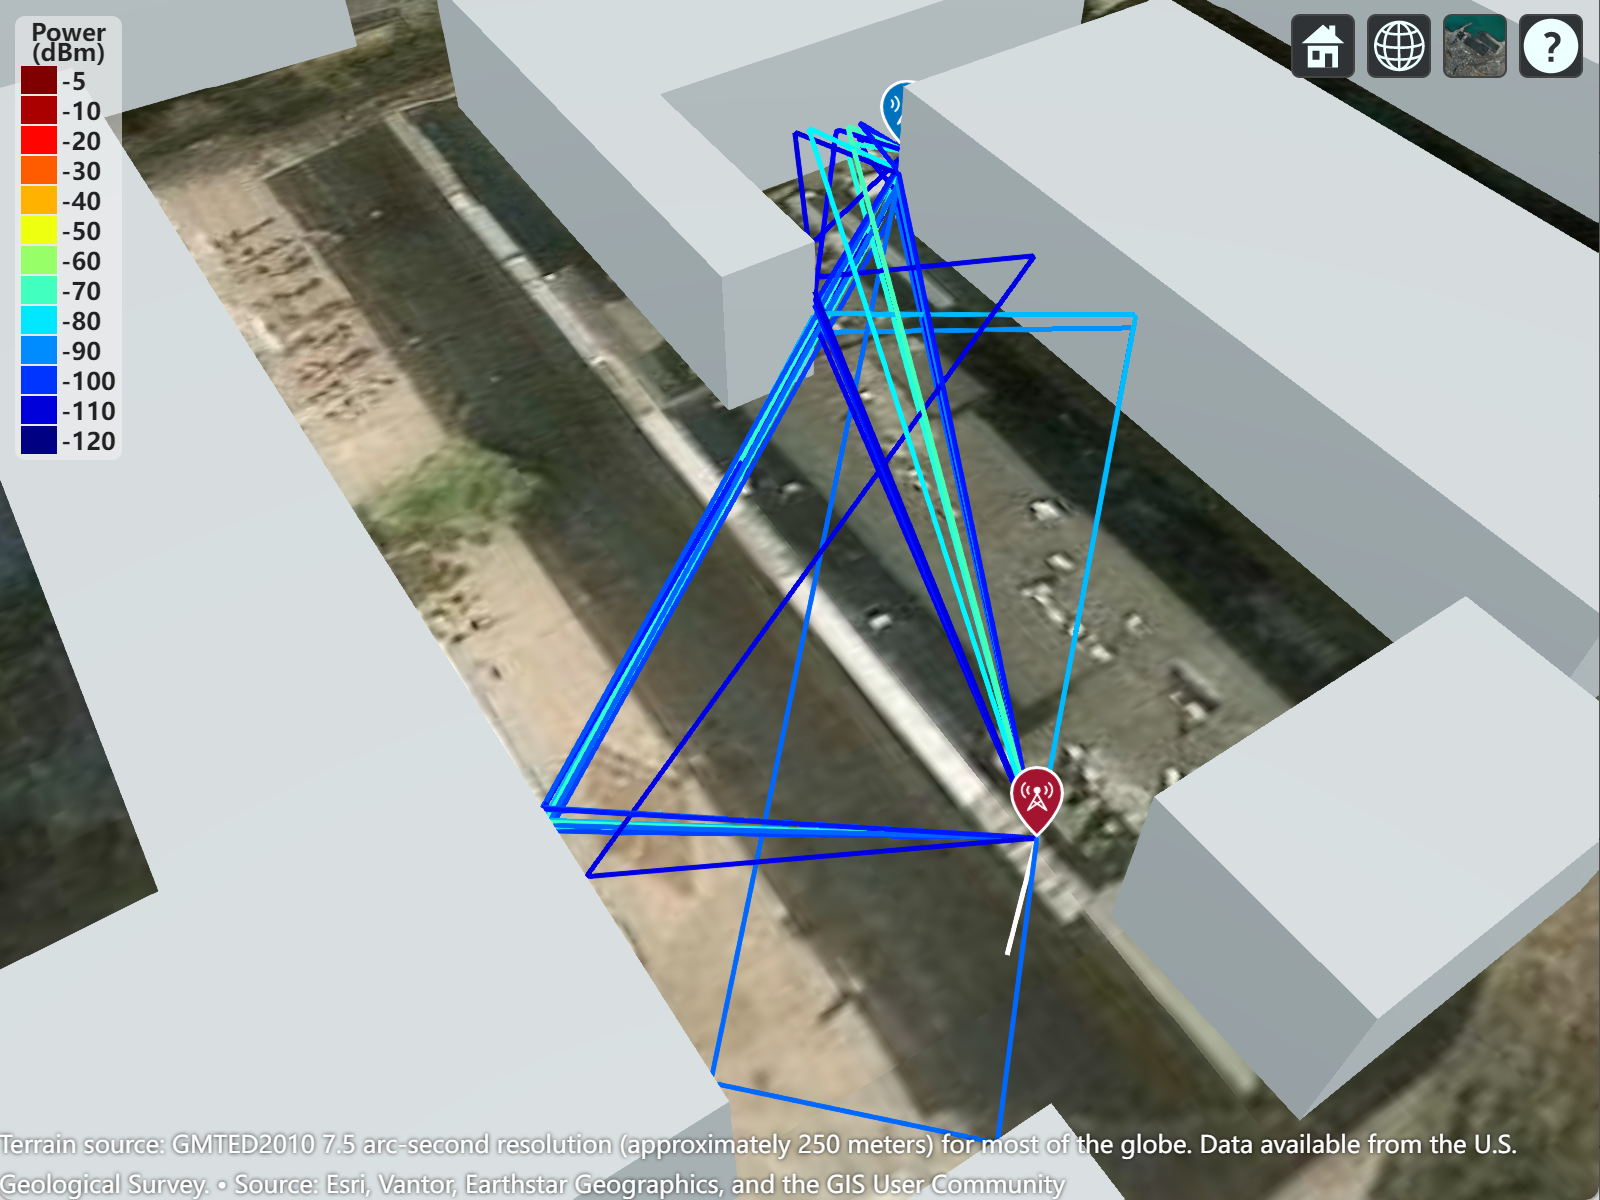
\includegraphics[width=.48\linewidth]{figures/school_step09.png}
\caption{混凝土、最多两次反射与一次衍射，含天气}
\end{figure}
增加衍射后，传播可绕过建筑边缘。\texttt{sigstrength}按复振幅相干合成，新增路径的相位可导致增强或抵消，因此“路径越多，接收功率必然越大”并不成立。本次结果表现为增强。

\section{相邻接收位置与带宽的影响}
\subsection{相邻接收天线的CIR}
两接收点仅相距0.222075 m，但在28 GHz下已相隔20.741个波长。基础代码采用混凝土、最多两次反射和一次衍射、low角间隔，不叠加天气损耗。
\begin{table}[H]\centering\small
\caption{相邻接收点的实际仿真结果}
\begin{tabular}{lrr}\toprule
接收点 & 接收功率/dBm & 几何射线数\\\midrule
Rx1 & $-62.189$ & 23\\
Rx2 & $-59.687$ & 24\\\bottomrule
\end{tabular}
\end{table}
\begin{figure}[H]\centering
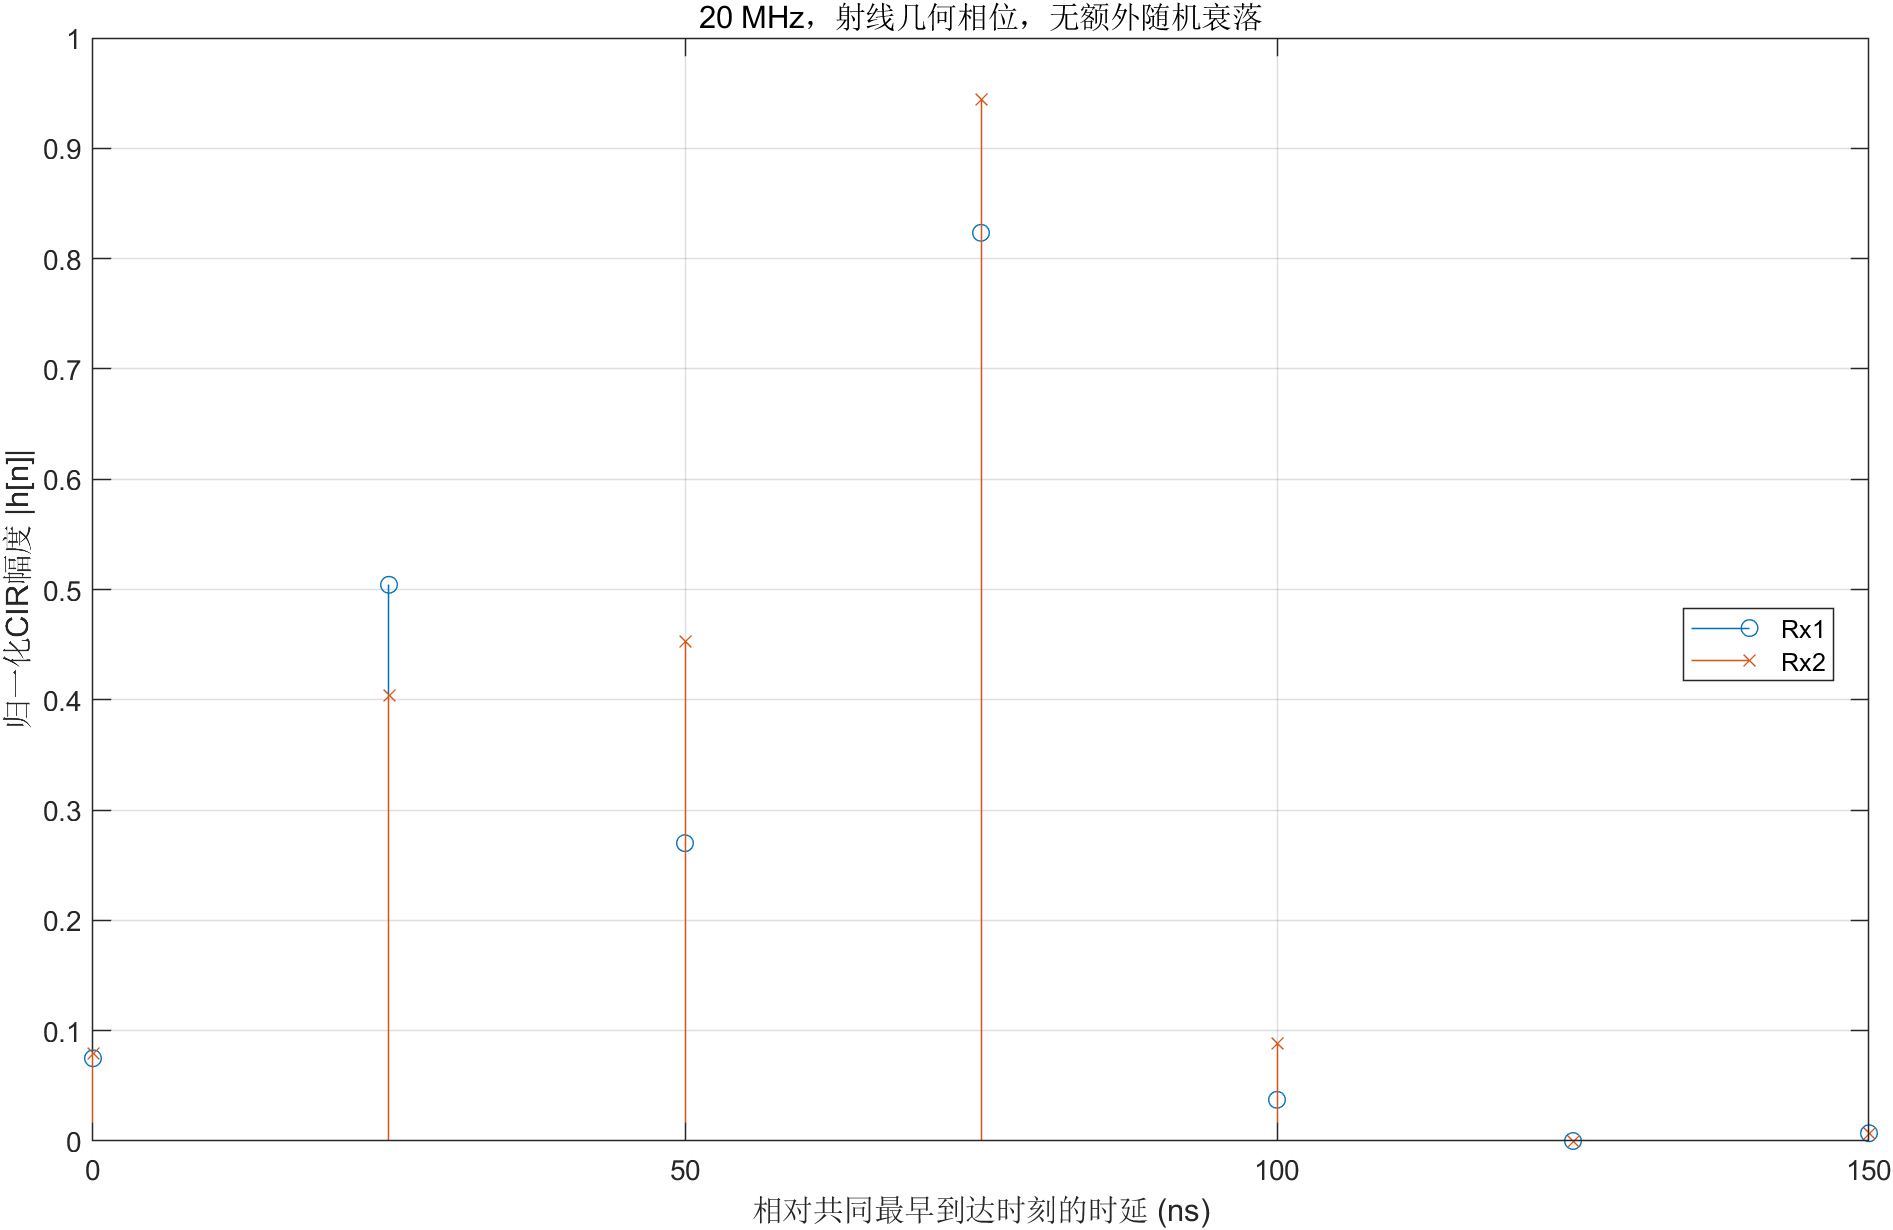
\includegraphics[width=.91\linewidth]{figures/CIR_position_rayphase.png}
\caption{相邻接收点的20 MHz CIR：使用射线几何相位}
\label{fig:cir-position}
\end{figure}
图\ref{fig:cir-position}的横轴为相对两个位置共同最早到达时刻的时延，单位为ns；纵轴为按各位置逐径功率和归一化后的复系数模值。两点的主抽头位置相近，均在约75 ns处出现最大幅度，但25、50和75 ns附近的幅度明显不同；Rx2的总接收功率比Rx1高\textbf{2.502 dB}。因此，相邻位置具有相似的主要时延结构，但射线路径、逐径相位及相干叠加结果并不相同。

基础代码还生成了独立复高斯随机系数下的CIR。该随机实现会改变抽头幅度及主峰位置。

\subsection{带宽对可分辨多径的影响}
固定Rx1的23条射线及同一组逐径随机复系数，仅改变带宽，得到表\ref{tab:bw}和图\ref{fig:bw}。
\begin{table}[H]\centering\small
\caption{带宽对比的实际结果与时延尺度}\label{tab:bw}
\begin{tabular}{lrrr}\toprule
带宽$B$/MHz & 20 & 40 & 80\\\midrule
采样间隔$T_s=1/(2B)$/ns & 25 & 12.5 & 6.25\\
分辨时间尺度$1/B$/ns & 50 & 25 & 12.5\\
几何射线数 & 23 & 23 & 23\\
占用时延格数 & 6 & 7 & 8\\\bottomrule
\end{tabular}
\end{table}
\begin{figure}[H]\centering
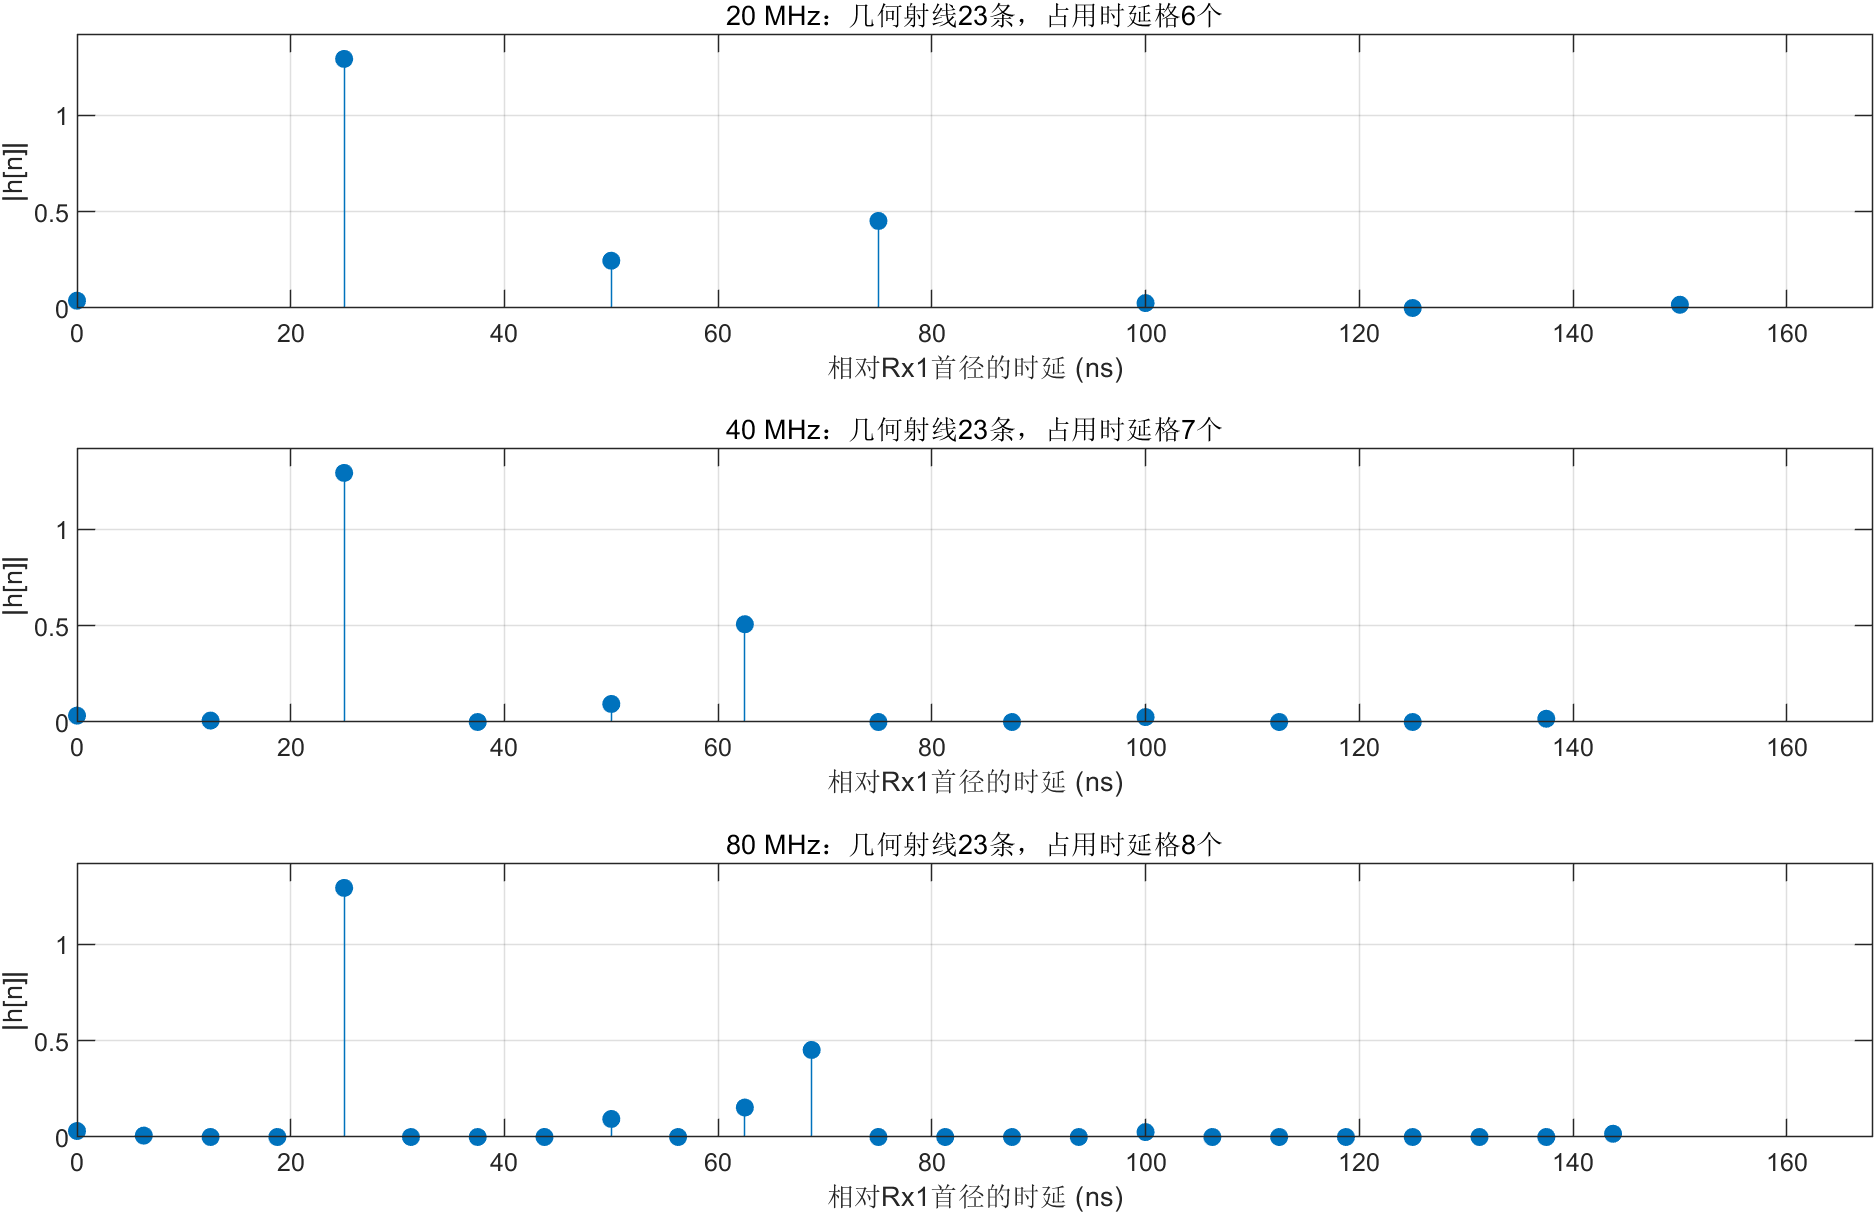
\includegraphics[width=.94\linewidth]{figures/CIR_bandwidth.png}
\caption{固定路径和随机系数时的20、40、80 MHz CIR对比}
\label{fig:bw}
\end{figure}
带宽增加后，时延网格变细，占用时延格由\textbf{6个增至7个、8个}。例如，20 MHz下约75 ns处的合成抽头，在80 MHz下可见约62.5 ns和68.75 ns附近的分离抽头。原本量化到同一格内的路径可被分配到不同抽头，其相干叠加方式也随之改变；这里并未新增几何传播路径。

因此，增大带宽通常有助于分离时延接近的多径。

\section{学校覆盖对比}
\begin{table}[H]\centering\small
\caption{两幅覆盖图的实际计算条件与耗时}
\begin{tabular}{lcccr}\toprule
条件 & 最大反射/衍射 & 角间隔 & 网格/m & 耗时/s\\\midrule
仅直射，完美反射材质，无天气 & 0/0 & medium & 3 & 6.982\\
混凝土，单次反射，含天气 & 1/0 & low & 2 & 74.489\\\bottomrule
\end{tabular}
\end{table}
\begin{figure}[H]\centering
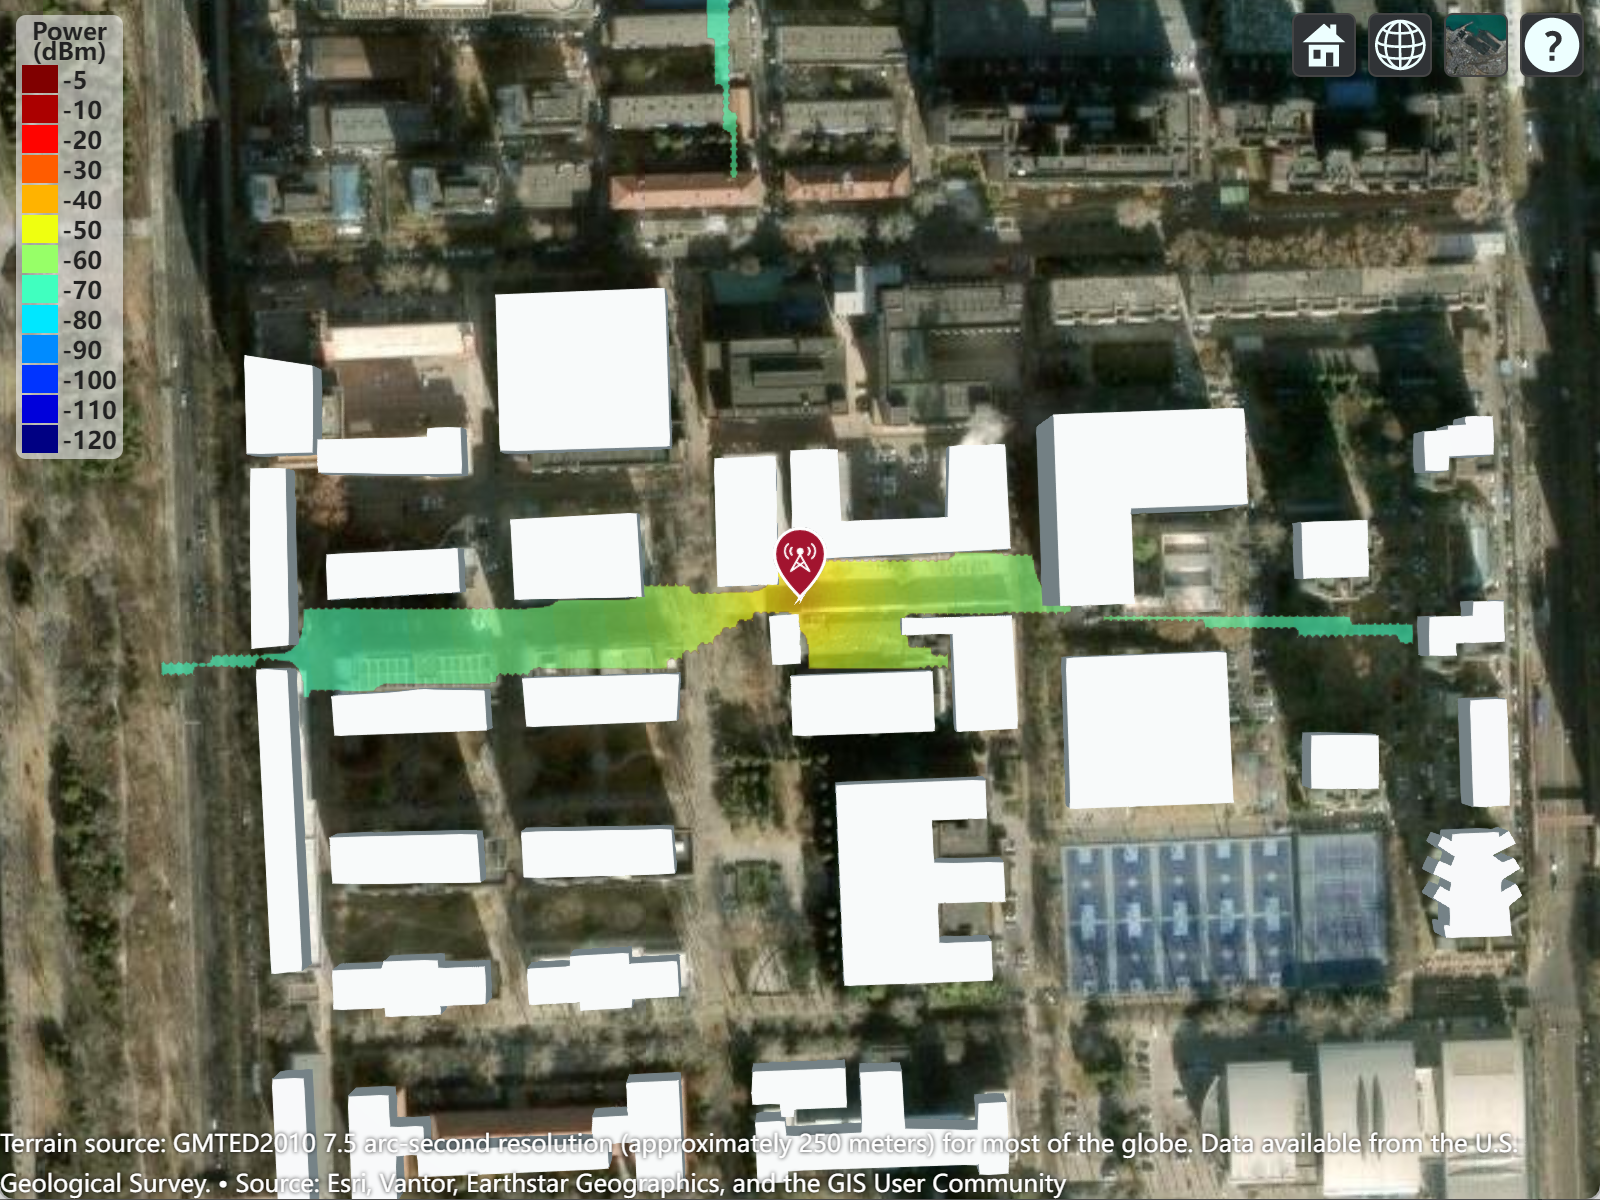
\includegraphics[width=.54\linewidth]{figures/school_step03.png}
\caption{仅直射覆盖：主要沿无遮挡道路分布}
\end{figure}
\begin{figure}[H]\centering
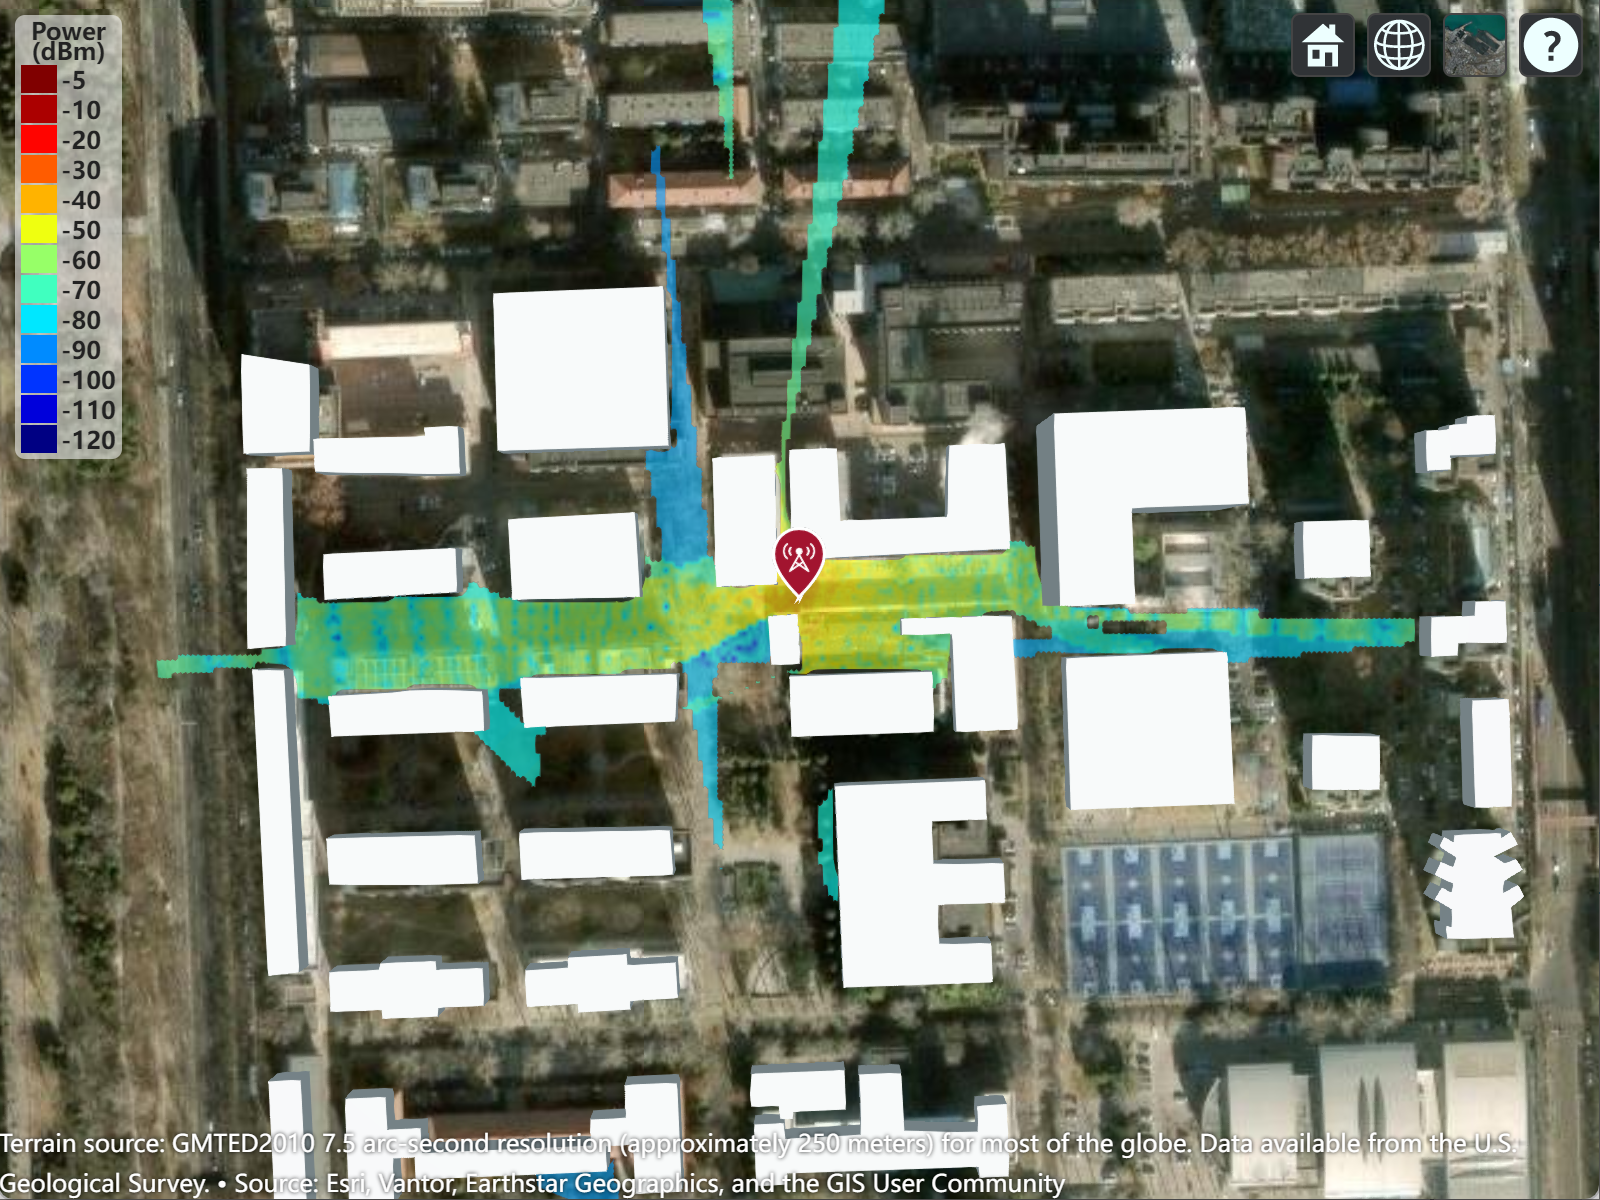
\includegraphics[width=.54\linewidth]{figures/school_step10.png}
\caption{单次反射并计入天气损耗的覆盖}
\end{figure}
两图采用相同的$[-120,-5]$ dBm色标及250 m计算范围。加入反射后，图中纵向支路及部分建筑周边出现更多有色区域，表明反射可以补充直射不可达的传播通道；局部颜色也受多径相干叠加影响。未着色区域不代表信号幅度严格为零。

\subsection{两次反射与一次衍射的预计算覆盖}
\begin{figure}[H]\centering
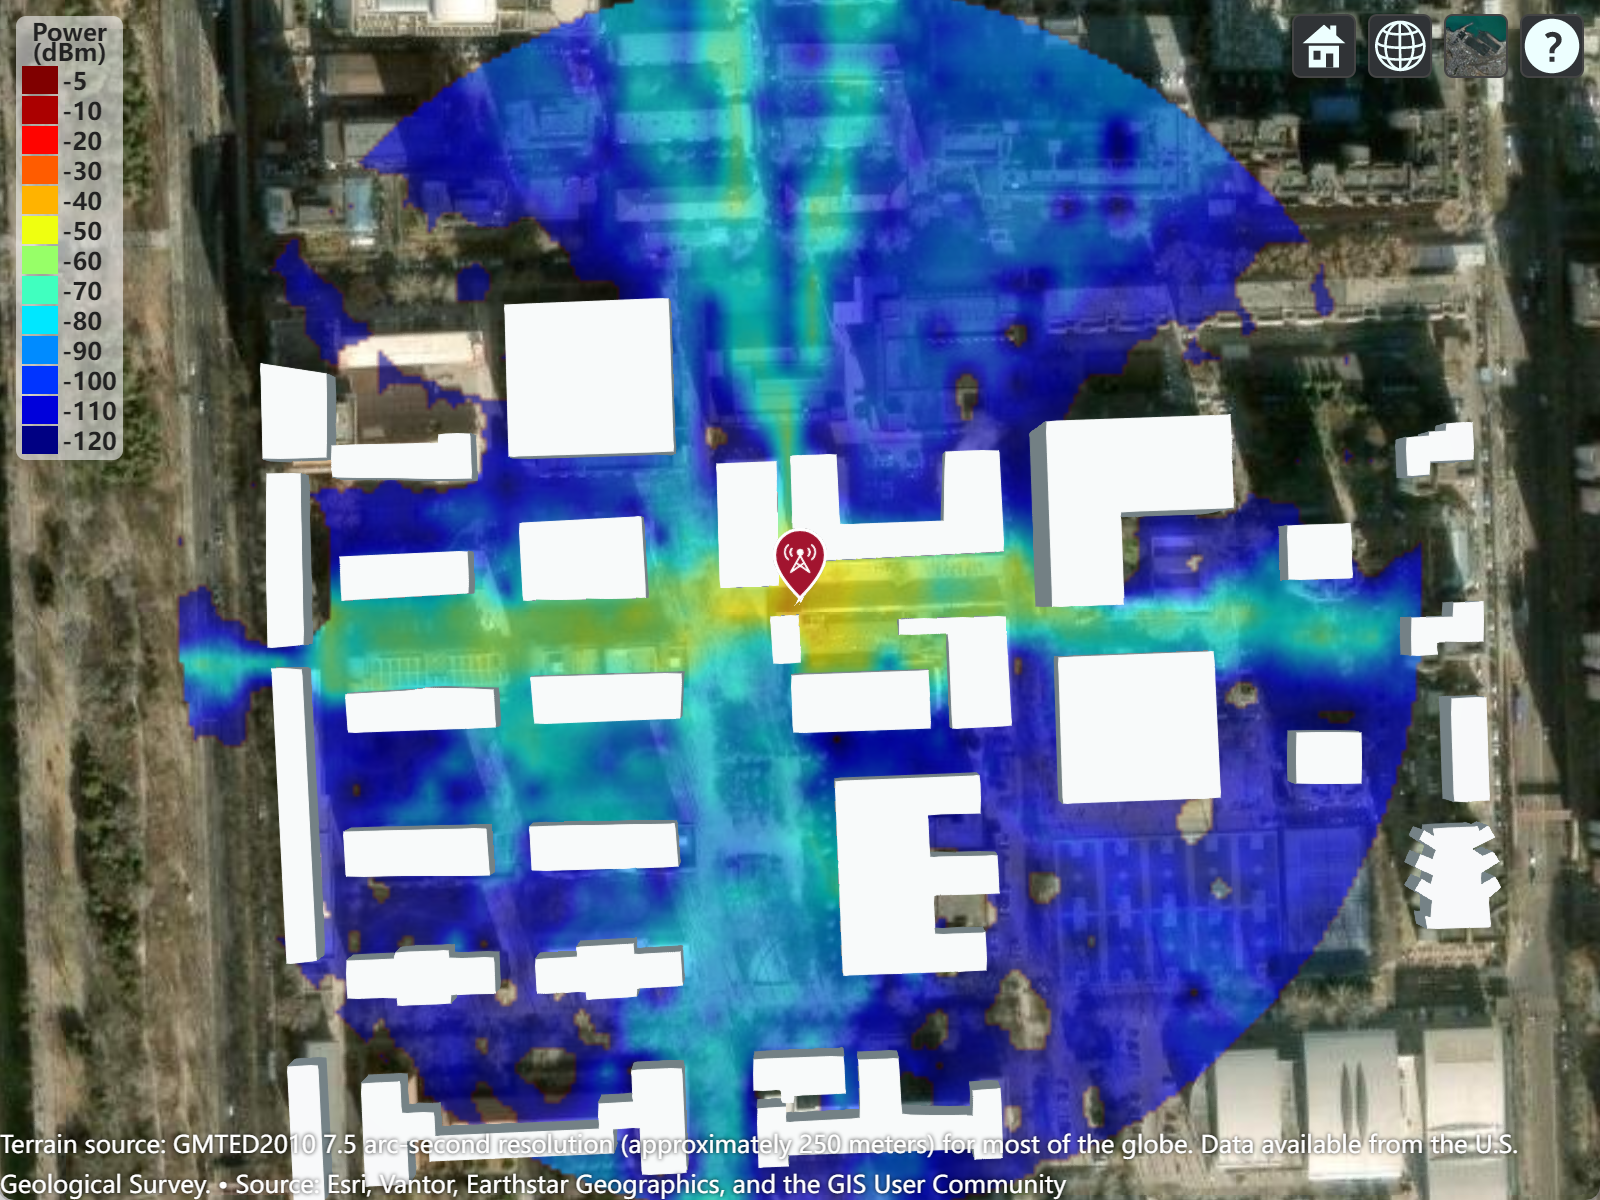
\includegraphics[width=.87\linewidth]{figures/school_step11.png}
\caption{步骤11：已有两次反射、一次衍射预计算覆盖结果的重绘}
\label{fig:coverage11}
\end{figure}
图\ref{fig:coverage11}由已有的\texttt{coverageResultsTwoRefOneDiff.mat}功率表加载绘制，共含1822个采样点，本轮未重新计算覆盖。与仅直射及单次反射图相比，主道路仍保持较强信号，更多建筑周边和遮挡区域出现蓝色弱信号区域，体现了更多间接传播通道对覆盖的补充作用。

\subsection{学校实验结论}
本次非视距链路中，改用混凝土引入7.602 dB的额外损耗，天气进一步引入0.584 dB损耗；扩大路径搜索后，更多反射、衍射路径改善了本次链路的合成接收功率。相邻接收点虽在空间上接近，仍可有不同射线数和CIR幅度。增大带宽使原有路径分布到更多离散时延格，改善时延区分能力，但不改变几何射线总数。

\section{社区场景}
\subsection{非视距链路、材质与天气}
社区场景选取玉泉北里住宅楼与商业中心之间的区域。发射点位于$(39.922250,116.245080)$，主接收点位于$(39.922540,116.244700)$（纬度、经度，单位为度）。保存的视线检查结果为主接收点LoS=0、近发射端检查点LoS=1。主链路由建筑遮挡，但周围墙面提供了间接传播通道。
\begin{table}[H]\centering\small
\caption{社区主接收点的链路结果}\label{tab:community-link}
\begin{tabular}{lccrrr}\toprule
条件 & 最大反射/衍射 & 角间隔 & 功率/dBm & 射线数 & 耗时/s\\\midrule
完美反射，无天气 & 1/0 & medium & $-63.028$ & 2 & 0.072\\
混凝土，无天气 & 1/0 & medium & $-70.995$ & 2 & 0.056\\
混凝土，含天气 & 1/0 & medium & $-72.089$ & 2 & 0.063\\
混凝土，含天气 & 2/0 & low & $-71.541$ & 6 & 0.128\\
混凝土，含天气 & 2/1 & low & $-71.134$ & 15 & 1.467\\\bottomrule
\end{tabular}
\smallskip\par\footnotesize 耗时口径同学校链路表，不含绘图；单次短任务计时不用于判断材质模型的计算复杂度。
\end{table}
\pair{community_step05.png}{社区：完美反射、最多一次反射}{community_step06.png}{社区：混凝土、最多一次反射}
更换材质后，两条路径的时延均保持为383.745 ns和714.679 ns，路损分别由102.608、108.010 dB增至110.554、116.025 dB，合成接收功率下降\textbf{7.967 dB}。路径不变，而材料反射损耗明显增加。

加入气体和降雨损耗后，功率进一步下降\textbf{1.095 dB}。两条路径分别增加0.876、1.631 dB路损，较长路径积累的天气衰减更大。

\subsection{反射与衍射路径}
\pair{community_step08.png}{社区：最多两次反射，含天气}{community_step09.png}{社区：最多两次反射、一次衍射，含天气}
最大反射数由1增至2、角间隔由medium改为low后，射线数由2增至6，合成接收功率增加0.548 dB。继续保持low并允许一次衍射后，共得到15条路径，其中\textbf{6条不含衍射、9条含一次衍射}，功率再增加0.408 dB，链路计算耗时约为原来的11.49倍。

加入衍射后，最早到达时延由383.745 ns提前到164.146 ns，说明绕过建筑边缘的路径可比原有反射绕行路线更短。

\subsection{相邻接收位置的CIR}
代码II保持混凝土、两反射一衍射、low角间隔，不叠加天气。Rx2位于$(39.922542,116.244700)$，与Rx1相距0.222069 m，约为20.741个波长。
\begin{table}[H]\centering\small
\caption{社区相邻接收点的实际结果}
\begin{tabular}{lrr}\toprule
接收点 & 接收功率/dBm & 几何射线数\\\midrule
Rx1 & $-69.868$ & 15\\
Rx2 & $-74.190$ & 15\\\bottomrule
\end{tabular}
\end{table}
\begin{figure}[H]\centering
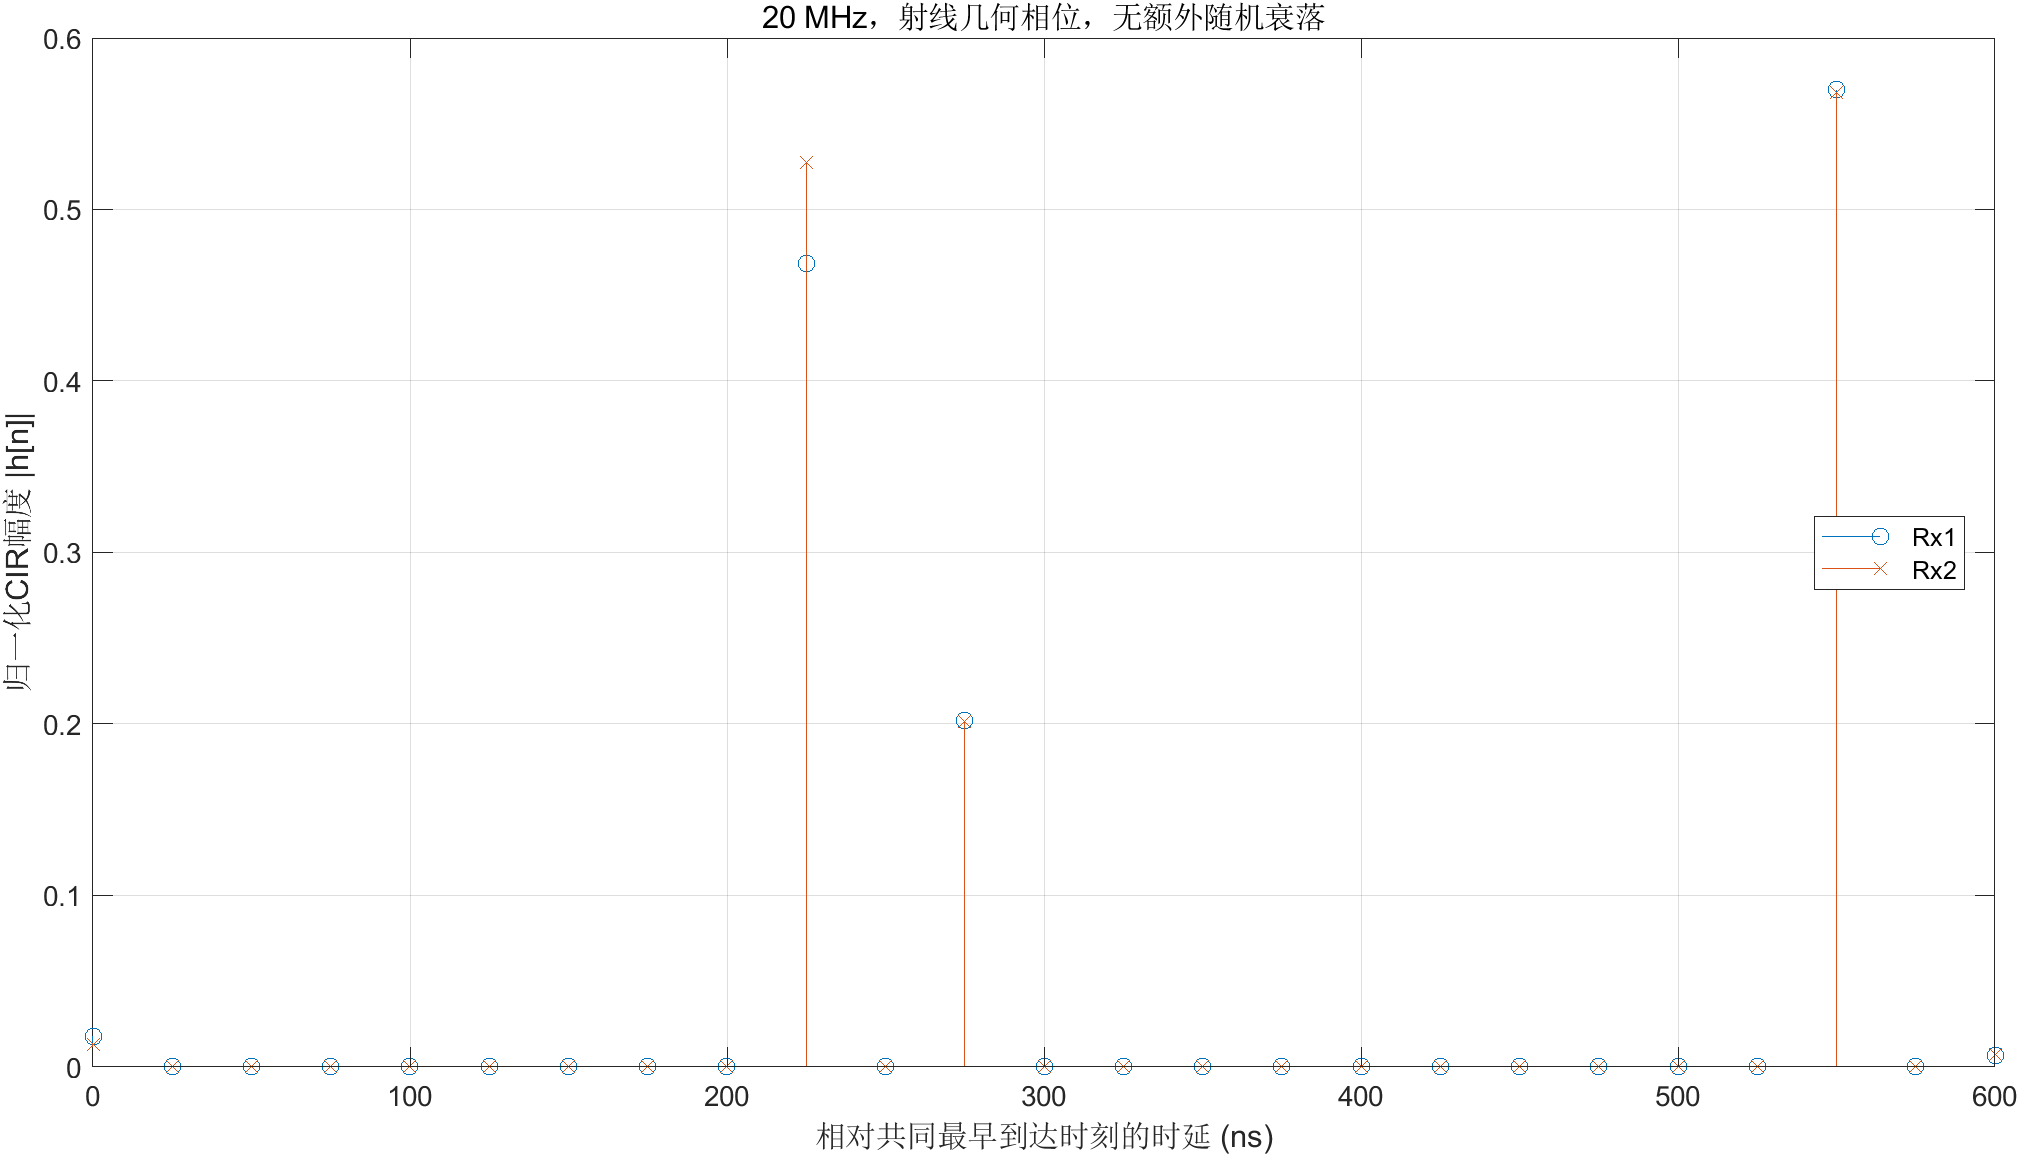
\includegraphics[width=.76\linewidth]{figures/community_CIR_position.png}
\caption{社区相邻接收点的20 MHz CIR：射线几何相位}
\label{fig:community-cir}
\end{figure}
两点的射线数相同，主要抽头均位于相对首径约225、275和550 ns处，但Rx2接收功率比Rx1低\textbf{4.322 dB}。图\ref{fig:community-cir}在225 ns处的归一化幅度约为0.469和0.527，550 ns处约为0.570和0.568。

\subsection{带宽影响}
固定Rx1的15条射线和同一组随机复系数，带宽对比如下。
\begin{table}[H]\centering\small
\caption{社区带宽对比结果}
\begin{tabular}{lrrr}\toprule
带宽$B$/MHz & 20 & 40 & 80\\\midrule
采样间隔$T_s$/ns & 25 & 12.5 & 6.25\\
分辨时间尺度$1/B$/ns & 50 & 25 & 12.5\\
几何射线数 & 15 & 15 & 15\\
占用时延格数 & 5 & 5 & 6\\\bottomrule
\end{tabular}
\end{table}
\begin{figure}[H]\centering
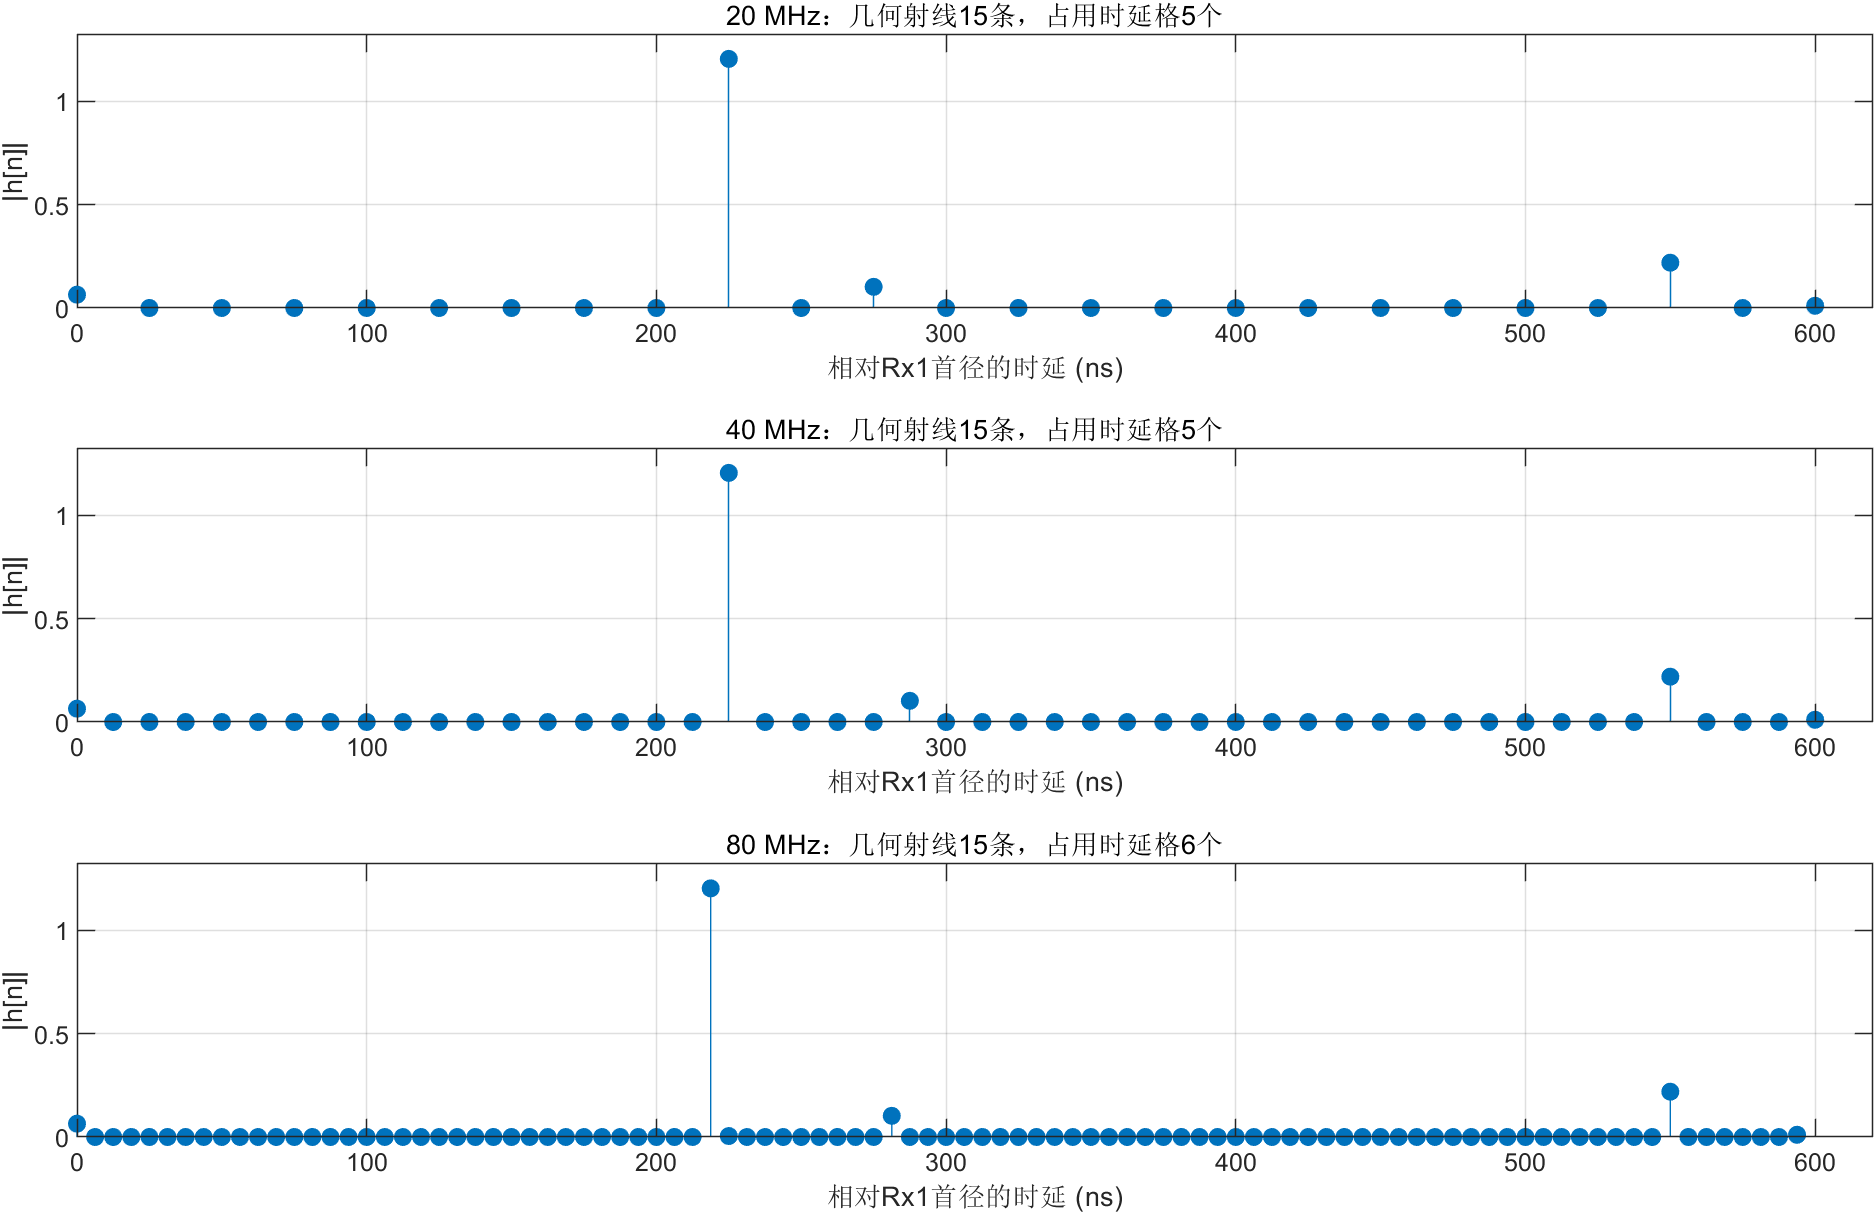
\includegraphics[width=.94\linewidth]{figures/community_CIR_bandwidth.png}
\caption{社区固定路径与随机系数时的20、40、80 MHz CIR}
\end{figure}
20 MHz增至40 MHz时，占用时延格仍为5个；增至80 MHz后才增加到6个。带宽变大使时延量化更细。

\subsection{覆盖对比}
\begin{table}[H]\centering\small
\caption{社区三种覆盖计算的条件与耗时}
\begin{tabular}{lcccr}\toprule
条件 & 最大反射/衍射 & 角间隔 & 网格/m & 耗时/s\\\midrule
仅直射，完美反射材质，无天气 & 0/0 & medium & 3 & 11.291\\
混凝土，单次反射，含天气 & 1/0 & low & 2 & 109.105\\
混凝土，两反射一衍射，含天气 & 2/1 & high & 10 & 155.835\\\bottomrule
\end{tabular}
\end{table}
\pair{community_step03.png}{社区仅直射覆盖}{community_step10.png}{社区单次反射并计入天气的覆盖}
\begin{figure}[H]\centering
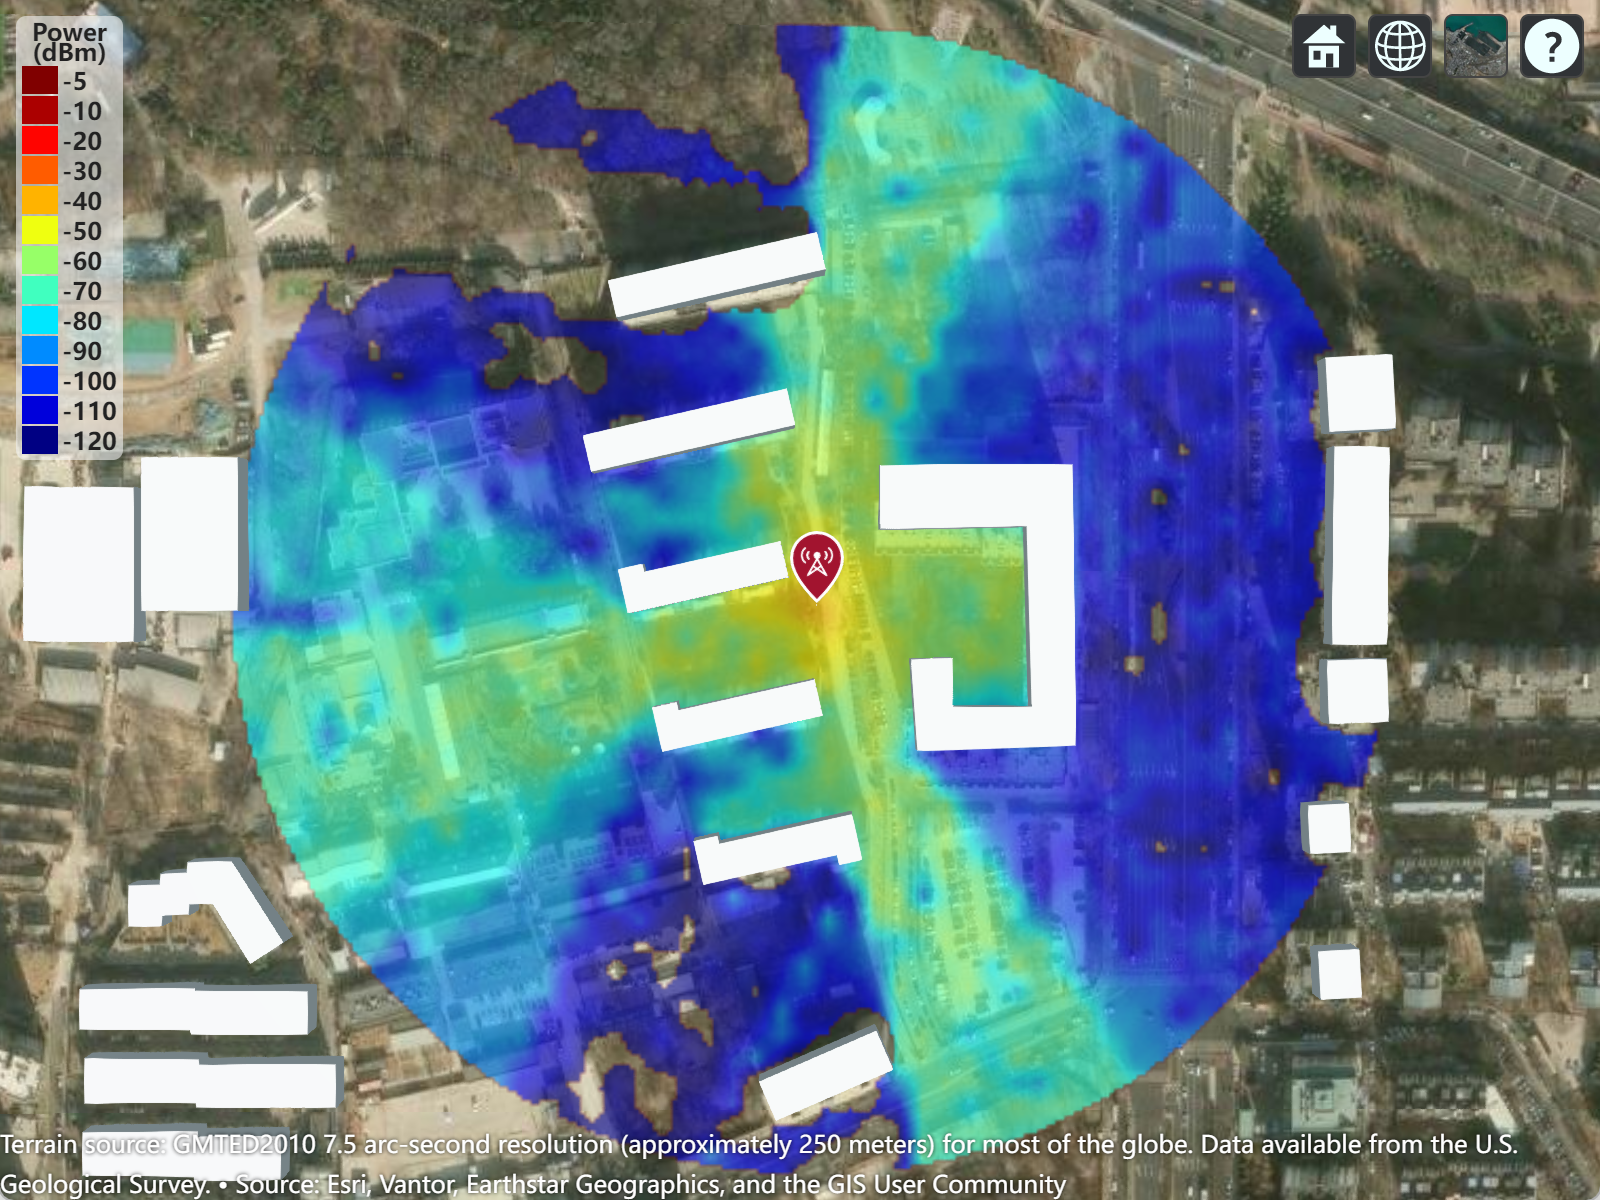
\includegraphics[width=.66\linewidth]{figures/community_step11.png}
\caption{社区两次反射、一次衍射并计入天气的覆盖}
\end{figure}
仅直射时，有色区域主要沿南北向空隙及部分楼间开口展开，住宅楼后方和商业中心背面存在明显阴影。单次反射增加了楼间通道的覆盖，并产生更明显的局部强弱变化；两反射一衍射条件下，更多楼后及商业中心另一侧出现蓝色弱信号区域，间接传播补充了原有阴影区。

\section{两场景对比与结论}
\begin{table}[H]\centering\small
\caption{学校与社区的主要结果对比}
\begin{tabular}{lrr}\toprule
指标 & 学校 & 社区\\\midrule
混凝土相对完美反射的附加损耗/dB & 7.602 & 7.967\\
单次反射链路的天气附加损耗/dB & 0.584 & 1.095\\
含天气、两反射一衍射接收功率/dBm & $-62.800$ & $-71.134$\\
同一条件下的几何射线数 & 23 & 15\\
增加衍射后的接收功率增量/dB & 1.080 & 0.408\\
20/40/80 MHz占用时延格数（无天气Rx1） & 6/7/8 & 5/5/6\\\bottomrule
\end{tabular}
\end{table}
两场景均表明，真实材质带来的约8 dB附加损耗比本次增加少量传播路径带来的功率增益更大。社区两条单反射路径的时延为383.745、714.679 ns，长于学校的236.797、278.868 ns；相同天气模型下，较长路径积累了更多衰减。

在两反射一衍射、含天气条件下，社区主链路比学校低8.334 dB。学校较多的射线也没有在所有带宽下转化成同样比例的可区分抽头。

相邻天线实验进一步说明，距离相近或射线数量相同都不足以保证CIR一致；带宽实验说明，增大带宽改善时延区分能力，但不增加几何传播路径。

\end{document}


